\documentclass{beamer}
 
\usepackage[utf8]{inputenc}
\usepackage{graphicx}
\usepackage{geometry}
\usepackage{layout}
\usepackage{siunitx}
\usepackage{hyperref}
\usepackage{float} 
 
%Information to be included in the title page:
\title{\textbf{Optimizing the Traveling Salesman Problem: Novel Approaches based on Renormalization Groups}}
\author{Benjamin Huang \& Shiye Su}
\institute{ISC 233/234}
\date{Spring 2017}
 
 
 
\begin{document}
 
\frame{\titlepage}
 
\begin{frame}
\frametitle{Background}
\begin{itemize}
\item Quasi-optimal solutions: solve many easy TSPs
\item Find new ways of grouping
\item Compare to other solutions
\item Find physical analogs
\end{itemize}
\begin{figure}[H]
  \centering
  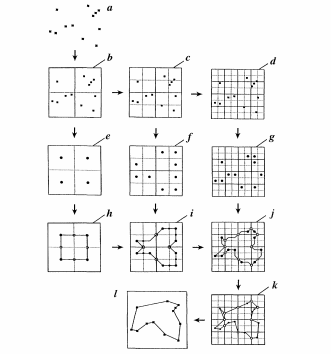
\includegraphics[width=.4\textwidth]{AlgGroup}
  \caption{Gridding method of renormalizing the commonwealth into megalopolis, as opposed to individual cities. }
  \label{fig:Grid}
\end{figure}
\end{frame}
 
\begin{frame}
  \frametitle{Lab Proposal}
\begin{itemize}
\item Grouping by reverse diffusion process
\item Radius of \textit{C. elegans}' chemotactic path 
\end{itemize}
\begin{figure}[H]
  \centering
  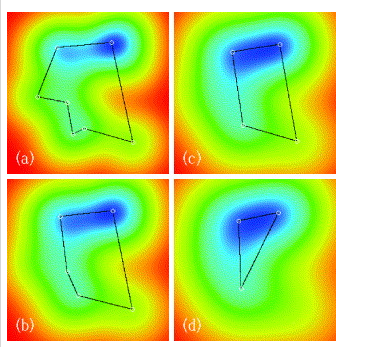
\includegraphics[width=.4\textwidth]{Blob.png}
  \caption{Diffusion as a physical analog to gridding}
\end{figure}
\end{frame}

\end{document}
